\documentclass{beamer}
\usetheme{Warsaw}
\usepackage[utf8]{inputenc}
\usepackage[french]{babel}
\usepackage[T1]{fontenc}
\usepackage{algorithm2e}
\usepackage{graphics}
\usepackage{subcaption} 
\title{Méthode PSO d’optimisation par Essaims de particules}
\author{Julien Choukroun \& Samy David \& Jessica Gourdon \& Luc Sagnes}
\institute{Polytech Nice Sophia} 
\date{29 Mai 2020} 

\begin{document}

\begin{frame}
  \titlepage
  \begin{figure}
    \begin{center}
      \includegraphics[scale=0.2]{../polytech.png} 
    \end{center}
  \end{figure}
\end{frame}

\begin{frame}
  \frametitle{Sommaire}
  \tableofcontents
\end{frame} 

\section{Introduction et motivations}
  \begin{frame}{Introduction}
    \begin{block}{\Large Présentation}
      \large Ce projet de fin de semestre consiste à étudier une métaheuristique :  l’optimisation par essaim particulaire (PSO).
    \end{block}\pause
    \begin{block}{\Large Objectif}
      \large L’objectif de cette méthode est de trouver l’optimum d’une fonction, c’est-à-dire le point vers lequel tous les éléments vont converger.
    \end{block}
  \end{frame}

  \begin{frame}{Optimisation}
    \begin{block}{\Large Problème d'optimisation}
      L’optimisation en mathématiques est la sélection d'un élément « meilleur » au vu de certains critères parmi un ensemble de solutions disponibles. \\ 
      Un problème d'optimisation consiste donc à maximiser ou minimiser une fonction réelle en choisissant en entrée des valeurs à partir d'un ensemble autorisé et en calculant la valeur de la fonction correspondante. Il faut noter que les problèmes de recherche de maximum ou de minimum sont symétriques. En effet, rechercher le minima de f revient à rechercher le maxima de -f. 
    \end{block}
  \end{frame}

  \begin{frame}{Métaheuristique}
    \begin{block}{\Large Définition}
      Une métaheuristique est un algorithme d’optimisation dont le but est de résoudre un problème d’optimisation difficile que l’on ne peut pas résoudre par le biais de méthodes d’optimisation classiques. \\
      Il existe de nombreux problèmes ne possédant pas de solution donnant un résultat en un temps raisonnable. \\
      Dans ce cas, nous pouvons avoir recours à des méthodes heuristiques. Il s’agit de méthodes permettant d’obtenir une solution approchée, la meilleure possible, dans un délai de temps raisonnable. \\
      Parmi celles-ci, il existe des algorithmes capables de s’adapter à une large gamme de problèmes d’optimisation différents. Il s’agit des métaheuristiques.
    \end{block}
  \end{frame}

  \begin{frame}{Principe de la PSO}
    \begin{block}{\Large Présentation}
      \large La PSO s’inspire du monde vivant. Elle se base sur la collaboration des individus entre eux pour converger progressivement vers un minimum global. Les individus seront appelés « particules ».  
    \end{block}\pause
    \begin{block}{\Large Objectif}
      \large Pour appliquer cette méthode, on doit définir un espace de recherche constitué de particules et une fonction à optimiser. Notre objectif est de déplacer ces particules afin qu’elles se retrouvent toutes très proches de l’optimum.
    \end{block}
  \end{frame}

  \begin{frame}{Principe de la PSO}
    \begin{block}{\Large Fonctionnement}
      \large Dans l’optimisation par essaim de particules, une équation permet de guider les particules. Le déplacement de celles-ci est influencé par trois composantes : 
 \\
•	L’inertie : la particule tend à suivre sa direction courante de déplacement 
\\
•	L’influence personnelle : la particule tend à se diriger vers la meilleure position par laquelle elle est déjà passée
\\
•	L’influence sociale : la particule tend à se diriger vers la meilleure position atteinte par ses voisines
    \end{block}
  \end{frame}

  \begin{frame}{Principe de la PSO}
    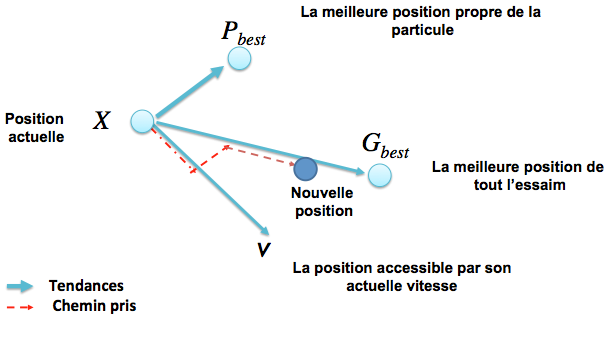
\includegraphics[scale=0.7]{../pso.png} 
  \end{frame}

\section{Algorithme}
  \begin{frame}{Algorithme}
    Une particule i de l’essaim dans un espace de dimension D est caractérisée, à l’instant t, par : \\
•	x : sa position dans l'espace de recherche \\
•	V : sa vitesse \\
•	xLB : la position de la meilleure solution par laquelle elle est passée, c'est le local best \\
•	xGB : la position de la meilleure solution connue de tout l’essaim, c'est le global best \\
•	f(xLB) : la valeur de sa meilleure solution \\
•	f(xGB) : la valeur de la meilleure solution connue de tout l’essaim \\
    Le déplacement de la particule i entre les itérations t et t+1 se fait selon les deux équations (1) et (2) suivantes \\
  \end{frame}

  \begin{frame}{Algorithme}
    \begin{block}{Calcul de la vitesse}
      $V_i^{t+1} = wV_i^t + \phi_1U_1^t(xLB_i^t-x_i^t) + \phi_2U_2^t(xGB_i^t-x_i^t) \quad (1)$
    \end{block}\pause
    \begin{block}{Calcul de la position}
      $x_i^{t+1} = x_i^t + V_i^{t+1} \quad (2)$
    \end{block}\pause
      w est la vitesse d'inertie. \\
      $\phi_1$ et $\phi_2$ sont des coefficients d'influence locale et globale. \\
      $U_1$ et $U_2$ sont des constantes aléatoires tirées dans l'intervalle [0;1] pour éviter une agglutination autour des global best.
  \end{frame}

  \begin{frame}{Algorithme}
    \scriptsize
    \begin{algorithm}[H]
      \SetAlgoLined
      \KwResult{Afficher la meilleure solution trouvée xGB }
      Initialisation des paramètres et de la taille N de l'essaim \\
      Initialisation des vitesses et des positions aléatoires des particules dans chaque dimension de l'espace de recherche \\
      Pour chaque particule, $xLB\gets x$ \\
      Calculer f(xLB) pour chaque particule \\
      Calculer xGB \emph{//le meilleur xLB} \\
      \While{Condition d'arret n'est pas vérifiée}{
        \For{i allant de 2 à N}{
           Calculer la nouvelle vitesse à l'aide de l'équation (1) \\
           Calculer la nouvelle position à l'aide de l'équation (2) \\
           Calculer f(xLB) pour chaque particule \\
        \If{f(x) est meilleure que f(xLB)}{
          $xLB\gets x$
        }
        \If{f(xLB) est meilleure que f(xGB)}{
         $xGB\gets xLB$
        }
        }
      }
    \end{algorithm}
  \end{frame}

\section{Test de validation}
  \begin{frame}{Test de validation}
    Nous avons étudier la fonction de Rosenbrock. \\
    Cette fonction se définit ainsi : \\
    $f(x) = \sum_{i=1}^{n-1}(100(x_{i+1}-x_i^2)^2 + (1-x_i)^2)$ \\
    Son domaine de recherche est $-\infty \le x_i \le +\infty$ avec $1 \le i \le n$ \\
    Son minimum global est : $f(1,1) = 0$ pour $n = 2$, $f(1,1,1) = 0$ pour $n = 3$ et $f(\underbrace{1,...,1}_{n fois}) = 0$ pour $n > 3$
    \begin{figure}
      \begin{center}
        \includegraphics[scale=0.15]{../Rosenbrock.jpg} 
      \end{center}
    \end{figure}
  \end{frame}

  \begin{frame}{Test de validation}
    \begin{block}{Paramètres}
      On choisit $w=1$, $\phi_1 = 1$ et $\phi_2 = 1$. \\
      On se place dans l'intervalle [-1000;1000]. \\
      On prend une population de 2000 et on étudie 1000 points, avec un nombre d'itérations maximales de 1000.
    \end{block}\pause
    \begin{figure}
      \begin{center}
        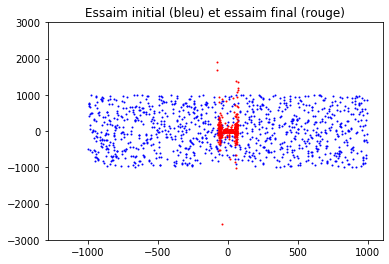
\includegraphics[scale=0.42]{../plotdebutfinal.png} 
      \end{center}
    \end{figure}
  \end{frame}

  \begin{frame}{Test de validation}
    \begin{figure}
      \begin{subfigure}[b]{0.49\textwidth}
        \includegraphics[width=\textwidth]{../plotdebut.png} 
      \end{subfigure}
      \begin{subfigure}[b]{0.49\textwidth}
        \includegraphics[width=\textwidth]{../plotfinal.png} 
      \end{subfigure}
    \end{figure}
  \end{frame}

\section{Etude paramétrique}
\subsection{Influence de la taille de l’essaim sur la convergence }
  \begin{frame}{Etude paramétrique selon la taille de l'essaim}
    \begin{block}{}
      \small Ici, on fait varier nos expériences en changeant la taille de l'essaim. Pour cela, dans chaque expérience nous gardons w=1, $\phi_1$=1 et $\phi_2$=1 . Cependant, la taille de l'essaim varie de 100 à 1000.
    \end{block}\pause
    \vspace{0.8 cm}
    \begin{tabular}{|c|c|c|c|}
      \hline
      \scriptsize Taille de l'essaim &\scriptsize  Xmin &\scriptsize f(Xmin) &\scriptsize Nombre d'itérations \\
\hline
      \scriptsize 100 &\scriptsize [1.02070949 ; 1.08213535] &\scriptsize 0.16273701 &\scriptsize 102\\
\hline
      \scriptsize 300 &\scriptsize [1.27860654 ; 1.63176694] &\scriptsize 0.07856271 & \scriptsize 70 \\
\hline
      \scriptsize 500 &\scriptsize [1.08377069 ; 1.17534695] &\scriptsize 0.00707963 &\scriptsize 40 \\
\hline
      \scriptsize 1000 &\scriptsize [1.08307939 ; 1.16752211] &\scriptsize 0.00997008 &\scriptsize 12 \\
      \hline
    \end{tabular}
  \end{frame}

  \begin{frame}{Observations de l'étude }
    \begin{block}{}
      Pour chaque test de notre expérience, nous avons gardé w=1,  $\phi_1$=1 et $\phi_2$=1. Nous avons fait varier la taille de l'essaim de 100 à 1000. \\
      Nous avons pu observé que lorsque la taille de l'essaim augmentait, le nombre d'itérations diminuait. \\
      Nous avons également observé que plus on augmentait la taille de l'essaim, plus la valeur de la fonction évaluée en notre Xmin (notre minimum) était proche de 0, qui est la valeur exacte minimale. \\
      Nous sommes donc amenés à supposer que lorsque la taille de l'essaim augmente, les particules convergent plus rapidement vers l'optimum. On a également une meilleure précision pour celui-ci.
    \end{block}
  \end{frame}

\subsection{Influence de $\phi_2$ dans PSO}
  \begin{frame}{Etude paramétrique selon $\phi_2$}
    \begin{block}{}
      \small Ici, on fait varier nos expériences en changeant notre valeur de $\phi_2$. Pour cela, dans chaque expérience nous gardons w=1 et $\phi_1$=1 et une taille de l'essaim égale à 500. Cependant, $\phi_2$ varie de 0.5 à 1.5.
    \end{block}\pause
    \vspace{0.8 cm}
    \begin{tabular}{|c|c|c|c|}
      \hline
      \scriptsize Valeur de $\phi_2$  & \scriptsize Xmin & \scriptsize f(Xmin) & \scriptsize Nombre d'itérations \\
      \hline
      \scriptsize 0.5 &\scriptsize  [0.97033649 ; 0.94606621] & \scriptsize0.00291691 &\scriptsize 55 \\
      \hline
      \scriptsize 0.7  & \scriptsize[0.94320374 ; 0.89711675]
 & \scriptsize 0.00882603 &\scriptsize 59 \\
      \hline
      \scriptsize 0.8 &\scriptsize [1.32667474 ; 1.71359502] &\scriptsize 0.32267037 &\scriptsize 12 \\
      \hline
      \scriptsize 1. &\scriptsize [0.91747737 ; 0.81736255]
 &\scriptsize 0.0663565 &\scriptsize 28 \\
      \hline
      \scriptsize 1.2 &\scriptsize [1. ; 1.] &\scriptsize 0. &\scriptsize 4 \\
      \hline
      \scriptsize 1.5 &\scriptsize [0.86023447 ; 0.74317104] &\scriptsize 0.02053783 &\scriptsize 69 \\
      \hline
    \end{tabular}
  \end{frame}

  \begin{frame}{Observations de l'étude }
    \begin{block}{}
      Pour chaque test de notre expérience, nous avons gardé w=1 et $\phi_1$=1 ainsi qu'une taille de l'essaim égale à 1000. Nous avons fait varier $\phi_2$ de 0.5 à 1.5. \\
      Nous avons pu observé qu'en augmentant $\phi_2$ jusqu'à la valeur 1.2, la nombre d'itérations diminuait (observation globale, malgré quelques écarts). \\
      Nous avons également observé qu'une fois que $\phi_2$ avait dépassé la valeur 1.2, le nombre d'itérations augmentait à nouveau. \\
      Nous sommes donc amenés à supposer que lorsque l'influence sociale augmente, les particules convergent plus rapidement vers l'optimum. Cependant, il existe une valeur limite pour cela. A partir de celle-ci, l'influence sociale devient trop importante par rapport aux autres influences pour une vitesse de convergence optimale.
     \end{block}
  \end{frame}

\section{Conclusion}
  \begin{frame}{Intérêts}
    \begin{block}{}
        Ce projet nous a permis de comprendre le fonctionnement de la PSO, méthode majeure utilisée dans de nombreux domaines, et susceptible de nous être utile au cours de notre vie professionnelle.
    \end{block}\pause
    \vspace{0.1 cm}
    \begin{block}{}
      Nous avons été particulièrement intéressés d’apprendre que des phénomènes naturels soient transformés sous forme mathématique afin d’être utilisés dans divers domaines.
    \end{block}\pause
    \vspace{0.1 cm}
    \begin{block}{}
      Il a également été intéressant de créer un algorithme permettant d’évaluer tous types de fonctions. Le fait de travailler sur un outil permettant de résoudre un large panel de problèmes suscite un intérêt particulier. 
    \end{block}
  \end{frame}

  \begin{frame}{Problèmes rencontrés}
    \begin{block}{}
      Tout d’abord, nous possédions des méthodes fonctionnant bien individuellement mais qui, une fois combinées avec d’autres, causaient des erreurs. 
    \end{block}\pause
    \vspace{0.1 cm}
    \begin{block}{}
      Nous nous sommes rendus compte que nous ne mémorisions pas assez d'éléments et de la mauvaise manière. En effet, lorsque nous mettions à jour nos nouveaux X, les anciens X que nous stockions se metaient également à jour. Nous avons donc dû utiliser deepcopy pour cela. Grâce à cela, nous faisions une véritable copie de l'élément et non pas un autre accès au même élément.
    \end{block}
  \end{frame}

  \begin{frame}{Problèmes rencontrés}
    \begin{block}{}
      Nous avons eu un problème lors de la création des constantes aléatoire $U_1$ et $U_2$. En effet, nous avons utilisé la fonction random de numpy : numpy.random.randn(1). Puis, lors des tests, nos valeurs étaient parfois abérrantes et nous avons vu que nos erreurs provenaient du random. Nous nous sommes donc tournés vers la fonction random.random() du module random.
    \end{block}\pause
    \begin{block}{}
      Nous avons finalement trouvé ce projet très intéressant avec, malgré des difficultés liées à la distance, une bonne cohésion d’équipe. 
    \end{block}
  \end{frame}

\section{Annexe}
  \begin{frame}{Annexe}
    \begin{figure}
      \begin{center}
        \includegraphics[scale=0.29]{../pythonPart1.png} 
      \end{center}
    \end{figure}
  \end{frame}

  \begin{frame}{Annexe}
    \begin{figure}
      \begin{center}
        \includegraphics[scale=0.29]{../pythonPart2.png} 
      \end{center}
    \end{figure}
  \end{frame}

  \begin{frame}{Annexe}
    \begin{figure}
      \begin{center}
        \includegraphics[scale=0.29]{../pythonPart3.png} 
      \end{center}
    \end{figure}
  \end{frame}

\end{document}